\documentclass[10pt,twocolumn]{article}

\usepackage[utf8]{inputenc}
\usepackage[T1]{fontenc}
\usepackage[margin=0.72in]{geometry}
\usepackage{amsmath,amssymb,amsfonts}
\usepackage{graphicx}
\usepackage{booktabs}
\usepackage{multirow}
\usepackage{xcolor}
\usepackage{hyperref}
\usepackage{caption}

\hypersetup{
    colorlinks=true,
    linkcolor=blue!60!black,
    citecolor=blue!60!black,
    urlcolor=blue!60!black
}

\title{\textbf{ABK-VLA: Task-ID-Free Continual Visuomotor Policy Learning via Autonomous B-Spline Knot Compression and Visual Prototype Routing}}

\author{
  Seungjoon Son \\
  Independent AI \& Robotics Researcher, Daejeon, Republic of Korea \\
  \texttt{https://github.com/5Color/abk-vla}
}

\date{November 2026}

\begin{document}

\maketitle

\begin{abstract}
Catastrophic forgetting remains a critical bottleneck for compact, real-time visuomotor policies deployed in sequential manipulation tasks. While large-scale foundation models mitigate forgetting through over-parameterization and cloud-scale data replay, lightweight closed-loop controllers suffer severe trajectory degradation when trained sequentially under strict memory and latency budgets. In this paper, we propose \textbf{ABK-VLA} (\textit{Autonomous B-spline Knot-based Visuomotor Policy}), evaluated on a goal-image-conditioned 2D multi-stroke drawing testbed that eliminates both experience replay buffers and inference-time \texttt{Task-ID} supervision. ABK-VLA compresses action chunks ($H=16$) into low-dimensional cubic B-spline control knots ($N_k=6$), allowing a frozen visual-spatial backbone ($4.59\text{M}$ shared parameters; $94.44\%$ of total $5.90\text{M}$ parameters frozen by $T_3$) to acquire new skills via compact 6-mode residual Winner-Take-All (WTA) slot heads ($0.33\text{M}$ trainable parameters per residual slot, $7.16\%$ of the backbone). At test time, a visual prototype router ($T=0.05$, zero task-routing heuristics) computes a $5{,}376$-dimensional hybrid Conv4-and-spatial target key and aggregates all slots via soft \textit{Select-then-Blend} residual composition. Evaluated across four sequential multi-stroke drawing tasks ($\text{apple} \rightarrow \text{sprout} \rightarrow \text{star} \rightarrow \text{cat}$), ABK-VLA achieves \textbf{99.98\% average diagonal routing confidence} ($4/4$ slot match on canonical targets), reduces forgetting from $89.33\%$ (naive fine-tuning) and $14.13\%$ (experience replay) down to \textbf{1.66\%}, and attains an average final $F_1$ of \textbf{85.59\%}---recovering \textbf{92.1\%} of an external-\texttt{Task-ID} Oracle policy ($92.96\%$) while improving geometric Chamfer Distance by $5.4\times$ ($0.0192$ vs.\ $0.1043$) and episode latency by $1.30\times$ ($464.3\text{ ms}$ vs.\ $601.6\text{ ms}$) over a recurrent GRU baseline.
\end{abstract}

\section{Introduction}
Real-world visuomotor agents must incrementally acquire new manipulation skills without erasing previously mastered behaviors. In large language and multimodal foundation models, massive parameter capacity and large-batch continual pre-training often dilute catastrophic forgetting. However, closed-loop visuomotor control policies operating on resource-constrained hardware cannot rely on billion-parameter backbones or unbounded replay buffers. When compact sequence-to-trajectory controllers are updated sequentially on new tasks, gradient interference overwrites shared motor representations, causing catastrophic trajectory collapse.

Existing parameter-isolation methods prevent weight interference by freezing task-specific subnetworks, yet they typically suffer from two limitations: (1) high per-task memory overhead when duplicating dense action decoders, and (2) reliance on an external oracle \texttt{Task-ID} during inference to activate the correct module.

To address both barriers in a controlled goal-image-conditioned motor benchmark, we introduce \textbf{ABK-VLA}:
\begin{itemize}
    \item \textbf{Compact B-Spline Parameter Isolation:} By representing $H=16$ continuous action chunks via $N_k=6$ cubic B-spline control knots, each new residual WTA slot requires $0.33\text{M}$ trainable parameters ($7.16\%$ of the $4.59\text{M}$ shared visual-state backbone), keeping $94.44\%$ of total model parameters frozen by $T_3$.
    \item \textbf{Task-ID-Free Visual Prototype Routing (Select-then-Blend):} During inference, ABK-VLA caches a $5{,}376$-dimensional hybrid Conv4-and-spatial target key per episode (\texttt{reset\_cache()}), computes temperature-scaled cosine similarity weights ($T=0.05$) without task-specific branching, and blends sequential residual slot outputs, achieving $99.98\%$ mean diagonal routing confidence across canonical target templates.
    \item \textbf{Horizon Alignment \& Post-Hoc Continuity:} Executing full $H=16$ chunks ($\text{exec\_steps}=16$) preserves pen-up jump landings across disconnected strokes, while post-hoc chunk-boundary $C^0/C^1$ smoothing yields low-jerk trajectories ($\text{NMJ}=3.33$).
\end{itemize}

\section{Related Work}
\textbf{Continual Learning (CL).} Classical CL approaches fall into regularization methods (e.g., EWC~\cite{kirkpatrick2017}), experience replay buffers, and parameter isolation (e.g., Progressive Networks~\cite{rusu2016}). While parameter isolation eliminates weight overwriting, standard implementations require explicit task identifiers at test time~\cite{farquhar2018}. ABK-VLA bridges this gap by pairing compact B-spline residual slots with autonomous visual prototype routing.

\textbf{Action Chunking \& Spline Visuomotor Policies.} Predicting temporal action chunks mitigates compounding error in imitation learning~\cite{zhao2023}. Parameterizing chunks as cubic B-splines reduces output dimensionality ($16\times 2 \rightarrow 6\times 2$) and enforces smooth intra-chunk trajectories, making slot-based continual expansion computationally practical.

\section{Methodology}

\subsection{Cubic B-Spline Trajectory Compression}
Given an action horizon $H=16$, rather than predicting $H$ independent $(x_t, y_t, p_t)$ waypoints, each slot $s \in \{0, \dots, K-1\}$ predicts $N_k=6$ spatial control knots $\mathbf{P}_{s,k} \in (0,1)^{N_k \times 2}$ (via sigmoid activation) across $M=6$ Winner-Take-All (WTA) modes $k \in \{0, \dots, M-1\}$, together with step-wise pen-contact logits $\mathbf{u}_{s,k} \in \mathbb{R}^{H}$ and mode selection logits $\mathbf{g}_s \in \mathbb{R}^M$. Using a precomputed clamped cubic B-spline basis matrix $\mathbf{B} \in \mathbb{R}^{H \times N_k}$, the continuous Cartesian trajectory $\hat{\mathbf{Y}} \in \mathbb{R}^{H \times 2}$ is reconstructed analytically via:
\begin{equation}
    \hat{\mathbf{Y}} = \mathbf{B}\mathbf{P},
\end{equation}
with a second-order control-point difference penalty $\mathcal{L}_{\text{smooth}} = \mathbb{E}[\|\mathbf{D}_2 \mathbf{P}\|_2^2]$ ($\lambda_{\text{sm}}=0.02$) suppressing intra-chunk loops. During closed-loop rollout, whenever both the previous executed step and the first predicted step are pen-down ($p_{t-1} > 0.5$ and $\hat{p}_0 > 0.5$), post-hoc boundary smoothing clamps $\hat{\mathbf{y}}_0 \leftarrow \mathbf{p}_{\text{prev}}$ ($C^0$) and blends $\hat{\mathbf{y}}_1 \leftarrow 0.7\,\hat{\mathbf{y}}_1 + 0.3\,(\mathbf{p}_{\text{prev}} + \mathbf{v}_{\text{prev}})$ whenever $\cos\alpha > 0$ ($C^1$ tangent continuity).

\subsection{Thin-Stroke Spatial Pointer \& Residual Cue}
To prevent thin 1\,px auxiliary strokes (e.g., stems, leaves, whiskers) from vanishing under spatial pooling, the policy derives two explicit residual cues from $\mathbf{M}_{\text{uncov}} = \max(0, \mathbf{I}_{\text{target}} - \mathbf{I}_{\text{canvas}})$:
\begin{enumerate}
    \item A $64$-dimensional residual map cue $\mathbf{c}_{\text{res}} = 4.0 \cdot \text{AvgPool}_{8\times 8}(\mathbf{M}_{\text{uncov}})$.
    \item A blended salience map for nearest-pixel localization:
    \begin{equation}
        \mathbf{M}_{\text{ptr}} = 0.7 \cdot \mathbf{M}_{\text{uncov}} + 0.3 \cdot \text{AvgPool}_{3\times 3}(\mathbf{M}_{\text{uncov}}),
    \end{equation}
    thresholded at $\mathbf{M}_{\text{ptr}} > 0.15$ (falling back to $\mathbf{M}_{\text{uncov}} > 0.08$ when empty) to locate the nearest uncovered pixel $(n_x, n_y)$, forming a $7$-dimensional geometric pointer $\mathbf{p}_{\text{geom}} = [c_x, c_y, r_{\text{rem}}, c_x - p_x, c_y - p_y, n_x - p_x, n_y - p_y]$.
\end{enumerate}
The $4$-stage ConvNet visual encoder ($4{,}583{,}168$ params, $256$-d output) and $2$-layer MLP state encoder ($4{,}416$ params, $64$-d output) form the $4.59\text{M}$-parameter shared backbone, concatenated with $\mathbf{c}_{\text{res}}$ and $\mathbf{p}_{\text{geom}}$ into a $391$-dimensional conditioning vector $\mathbf{h}_{\text{cond}}$.

\subsection{Dynamic Residual Slot Expansion \& Select-then-Blend}
To resolve stroke-order multimodality and cross-task transfer, slot $0$ predicts base control knots directly while each expanded slot $s > 0$ (\texttt{ResidualWTASlotHead}, $328{,}367$ params) predicts logit-space residuals $(\Delta \mathbf{P}_s, \Delta \mathbf{u}_s)$ modulated by a learnable scalar gate $\alpha_s$ (\texttt{prior\_weight}, initialized at $1.0$):
\begin{equation}
    \tilde{\mathbf{P}}_s = \sigma\!\Big(\alpha_s \cdot \operatorname{logit}\big(\operatorname{clip}(\bar{\mathbf{P}}_{<s}, 0.05, 0.95)\big) + \Delta \mathbf{P}_s\Big),
\end{equation}
\begin{equation}
    \tilde{\mathbf{u}}_s = \alpha_s \cdot \operatorname{clip}(\bar{\mathbf{u}}_{<s}, -2.5, 2.5) + \Delta \mathbf{u}_s,
\end{equation}
where $(\bar{\mathbf{P}}_{<s}, \bar{\mathbf{u}}_{<s})$ is the softmax-weighted output of slots $0, \dots, s-1$. Each slot's mode selector \texttt{sel\_head} directly concatenates the $7$-d $\mathbf{p}_{\text{geom}}$ to its trunk features ($256 + 7 \rightarrow 128 \rightarrow M$).

\textbf{Hybrid 5,376-d Prototype Key \& Novelty Detection.} Given target image $\mathbf{I}_{\text{target}}$, \texttt{\_compute\_target\_key} extracts the $L_2$-normalized Conv4 spatial feature map ($4\times 4 \times 256 = 4{,}096$-d) weighted by $0.5$ and concatenates it with $L_2$-normalized multi-scale target silhouette average pooling ($32\times 32$ smoothed + $16\times 16 = 1{,}280$-d) weighted by $1.0$, followed by global $L_2$ normalization into $\mathbf{z} \in \mathbb{R}^{5{,}376}$. By construction, squared $L_2$ energy is split $80\% / 20\%$ between multi-scale spatial target pooling and Conv4 features. At task transitions during training, if $\max_{j < K} \mathbf{z}_\tau^\top \boldsymbol{\mu}_j < \gamma$ ($\gamma = 0.85$), a new residual slot $K$ is instantiated, $\boldsymbol{\mu}_K \leftarrow \mathbf{z}_\tau$ is registered, and the shared backbone ($4.59\text{M}$) plus all prior slots are permanently frozen (in \texttt{eval()} mode to lock BatchNorm statistics). After $T_0$, \texttt{refresh\_slot\_key} updates $\boldsymbol{\mu}_0$ prior to backbone freezing.

\textbf{Training Objective.} Active slot $s$ is trained without \texttt{Task-ID} using $M=6$ WTA supervision over trajectory $L_1$, control-point $L_1$, smoothness, and transition-weighted pen BCE (\texttt{balanced\_pen\_transition\_loss}), combined with a $6.0\times$ inverse-frequency focal gating loss on air-flight/transition chunks and pen-consistent gating supervision:
\begin{equation}
    \mathcal{L}_D = 0.90\,\mathcal{L}_{\text{win}} + 0.05\,\mathcal{L}_{\text{all}} + 0.10\,\mathcal{L}_{\text{focal\_gate}} + 0.10\,\mathcal{L}_{\text{pen\_exp}}.
\end{equation}

\textbf{Select-then-Blend Inference.} At test time, without any \texttt{Task-ID}, routing weights $\mathbf{w} \in \Delta^{K-1}$ are computed once per episode via cached static keys (\texttt{reset\_cache()}, $T = 0.05$):
\begin{equation}
    w_s = \frac{\exp(\mathbf{z}^\top \boldsymbol{\mu}_s / T)}{\sum_{j=0}^{K-1} \exp(\mathbf{z}^\top \boldsymbol{\mu}_j / T)}.
\end{equation}
Rather than hard \texttt{argmax} routing over a single slot, ABK-VLA executes \textit{Select-then-Blend}: within each slot $s \in \{0, \dots, K-1\}$, \texttt{argmax} selects the best mode $k_s^* = \arg\max_k g_{s,k}$, residual composition chains sequentially across slots, and the final control knots and pen logits are blended across all slots as $\mathbf{P}^* = \operatorname{clip}(\sum_{s=0}^{K-1} w_s \tilde{\mathbf{P}}_{s,k_s^*}, 0, 1)$ and $\mathbf{u}^* = \sum_{s=0}^{K-1} w_s \tilde{\mathbf{u}}_{s,k_s^*}$.

\section{Experimental Setup}

\subsection{5-Model Continual Learning Protocol}
All experiments were conducted on Intel(R) Arc Graphics (\texttt{xpu}, FP32, PyTorch \texttt{2.15.0+xpu}, \texttt{seed=42}) across four sequential multi-stroke drawing tasks: $T_0(\text{apple}) \rightarrow T_1(\text{sprout}) \rightarrow T_2(\text{star}) \rightarrow T_3(\text{cat})$. Models~1--5 share identical episode-level train/val splits ($85\% / 15\%$), identical affine/elastic/covariate-shift augmentation schedules ($T_0$: $10\text{ epochs} \times 1\times$; $T_1$: $12\text{ epochs} \times 3\times$; $T_2$: $12\text{ epochs} \times 5\times$; $T_3$: $16\text{ epochs} \times 5\times$; batch size $64$; \texttt{WeightedRandomSampler} with $2.0\times$ secondary-stroke and $2.5\times$ jump-chunk weights on multi-stroke tasks), identical spatial pointers, post-hoc $C^0/C^1$ smoothing, and identical rollout parameters ($\text{exec\_steps}=16$, $\text{max\_iters}=100$, base $\text{patience}=8$, dynamically extended to $\text{effective\_patience}=16$ when $>5\%$ target ink remains, with stale accumulation throttled $1/3$ during air flights):
\begin{enumerate}
    \item \textbf{Model 1 (GRU + Naive FT):} Autoregressive $(x, y, p)$ GRUCell baseline trained sequentially at $\text{lr}=3\times 10^{-4}$ without isolation or replay.
    \item \textbf{Model 2 (ABK + Naive FT):} Single-mode B-spline MLP policy trained sequentially at $\text{lr}=3\times 10^{-4}$ with $\text{pen\_up\_weight}=2.0$ BCE.
    \item \textbf{Model 3 (ABK + Replay):} Model~2 augmented with a balanced replay buffer ($256$ samples/task) at $\text{lr}=3\times 10^{-4}$.
    \item \textbf{Model 4 (Oracle Slots / Model C):} Multi-slot 6-mode \texttt{WTASlotHead} ($0.30\text{M}$/slot) supplied with ground-truth \texttt{Task-ID} labels at test time ($\text{lr}=10^{-3}$ for $T_1$--$T_3$, cross-entropy gate loss).
    \item \textbf{Model 5 (Autonomous ABK-VLA / Model D, Ours):} Replay-free, \texttt{Task-ID}-free residual WTA policy ($0.33\text{M}$/slot, $\text{lr}=10^{-3}$ for $T_1$--$T_3$, $5\times 10^{-3}$ on $\alpha_s$) with focal and pen-consistent gating supervision.
\end{enumerate}

\subsection{Evaluation Metrics}
Let $R_{i,t}$ denote the pixel-level $F_1$ score ($\text{tol}=2$\,px) on task $i$ immediately after training on task $t$. We report standard Continual Learning Forgetting Rate ($\text{FR}$) and Backward Transfer ($\text{BWT}$):
\begin{equation}
    \text{FR} = \frac{1}{K-1} \sum_{i=0}^{K-2} \max\!\left(0,\; \max_{t \in \{i, \dots, K-2\}} R_{i,t} - R_{i, K-1}\right),
\end{equation}
\begin{equation}
    \text{BWT} = \frac{1}{K-1} \sum_{i=0}^{K-2} \big(R_{i, K-1} - R_{i,i}\big),
\end{equation}
alongside symmetric \textbf{Chamfer Distance (CD $\downarrow$)}, pen-down \textbf{Normalized Mean Jerk (NMJ $\downarrow$)}, connected \textbf{Component Recall (CR $\uparrow$)}, and per-episode \textbf{Inference Latency (ms $\downarrow$)}.

\section{Results and Diagnostic Analysis}

\begin{figure*}[t]
    \centering
    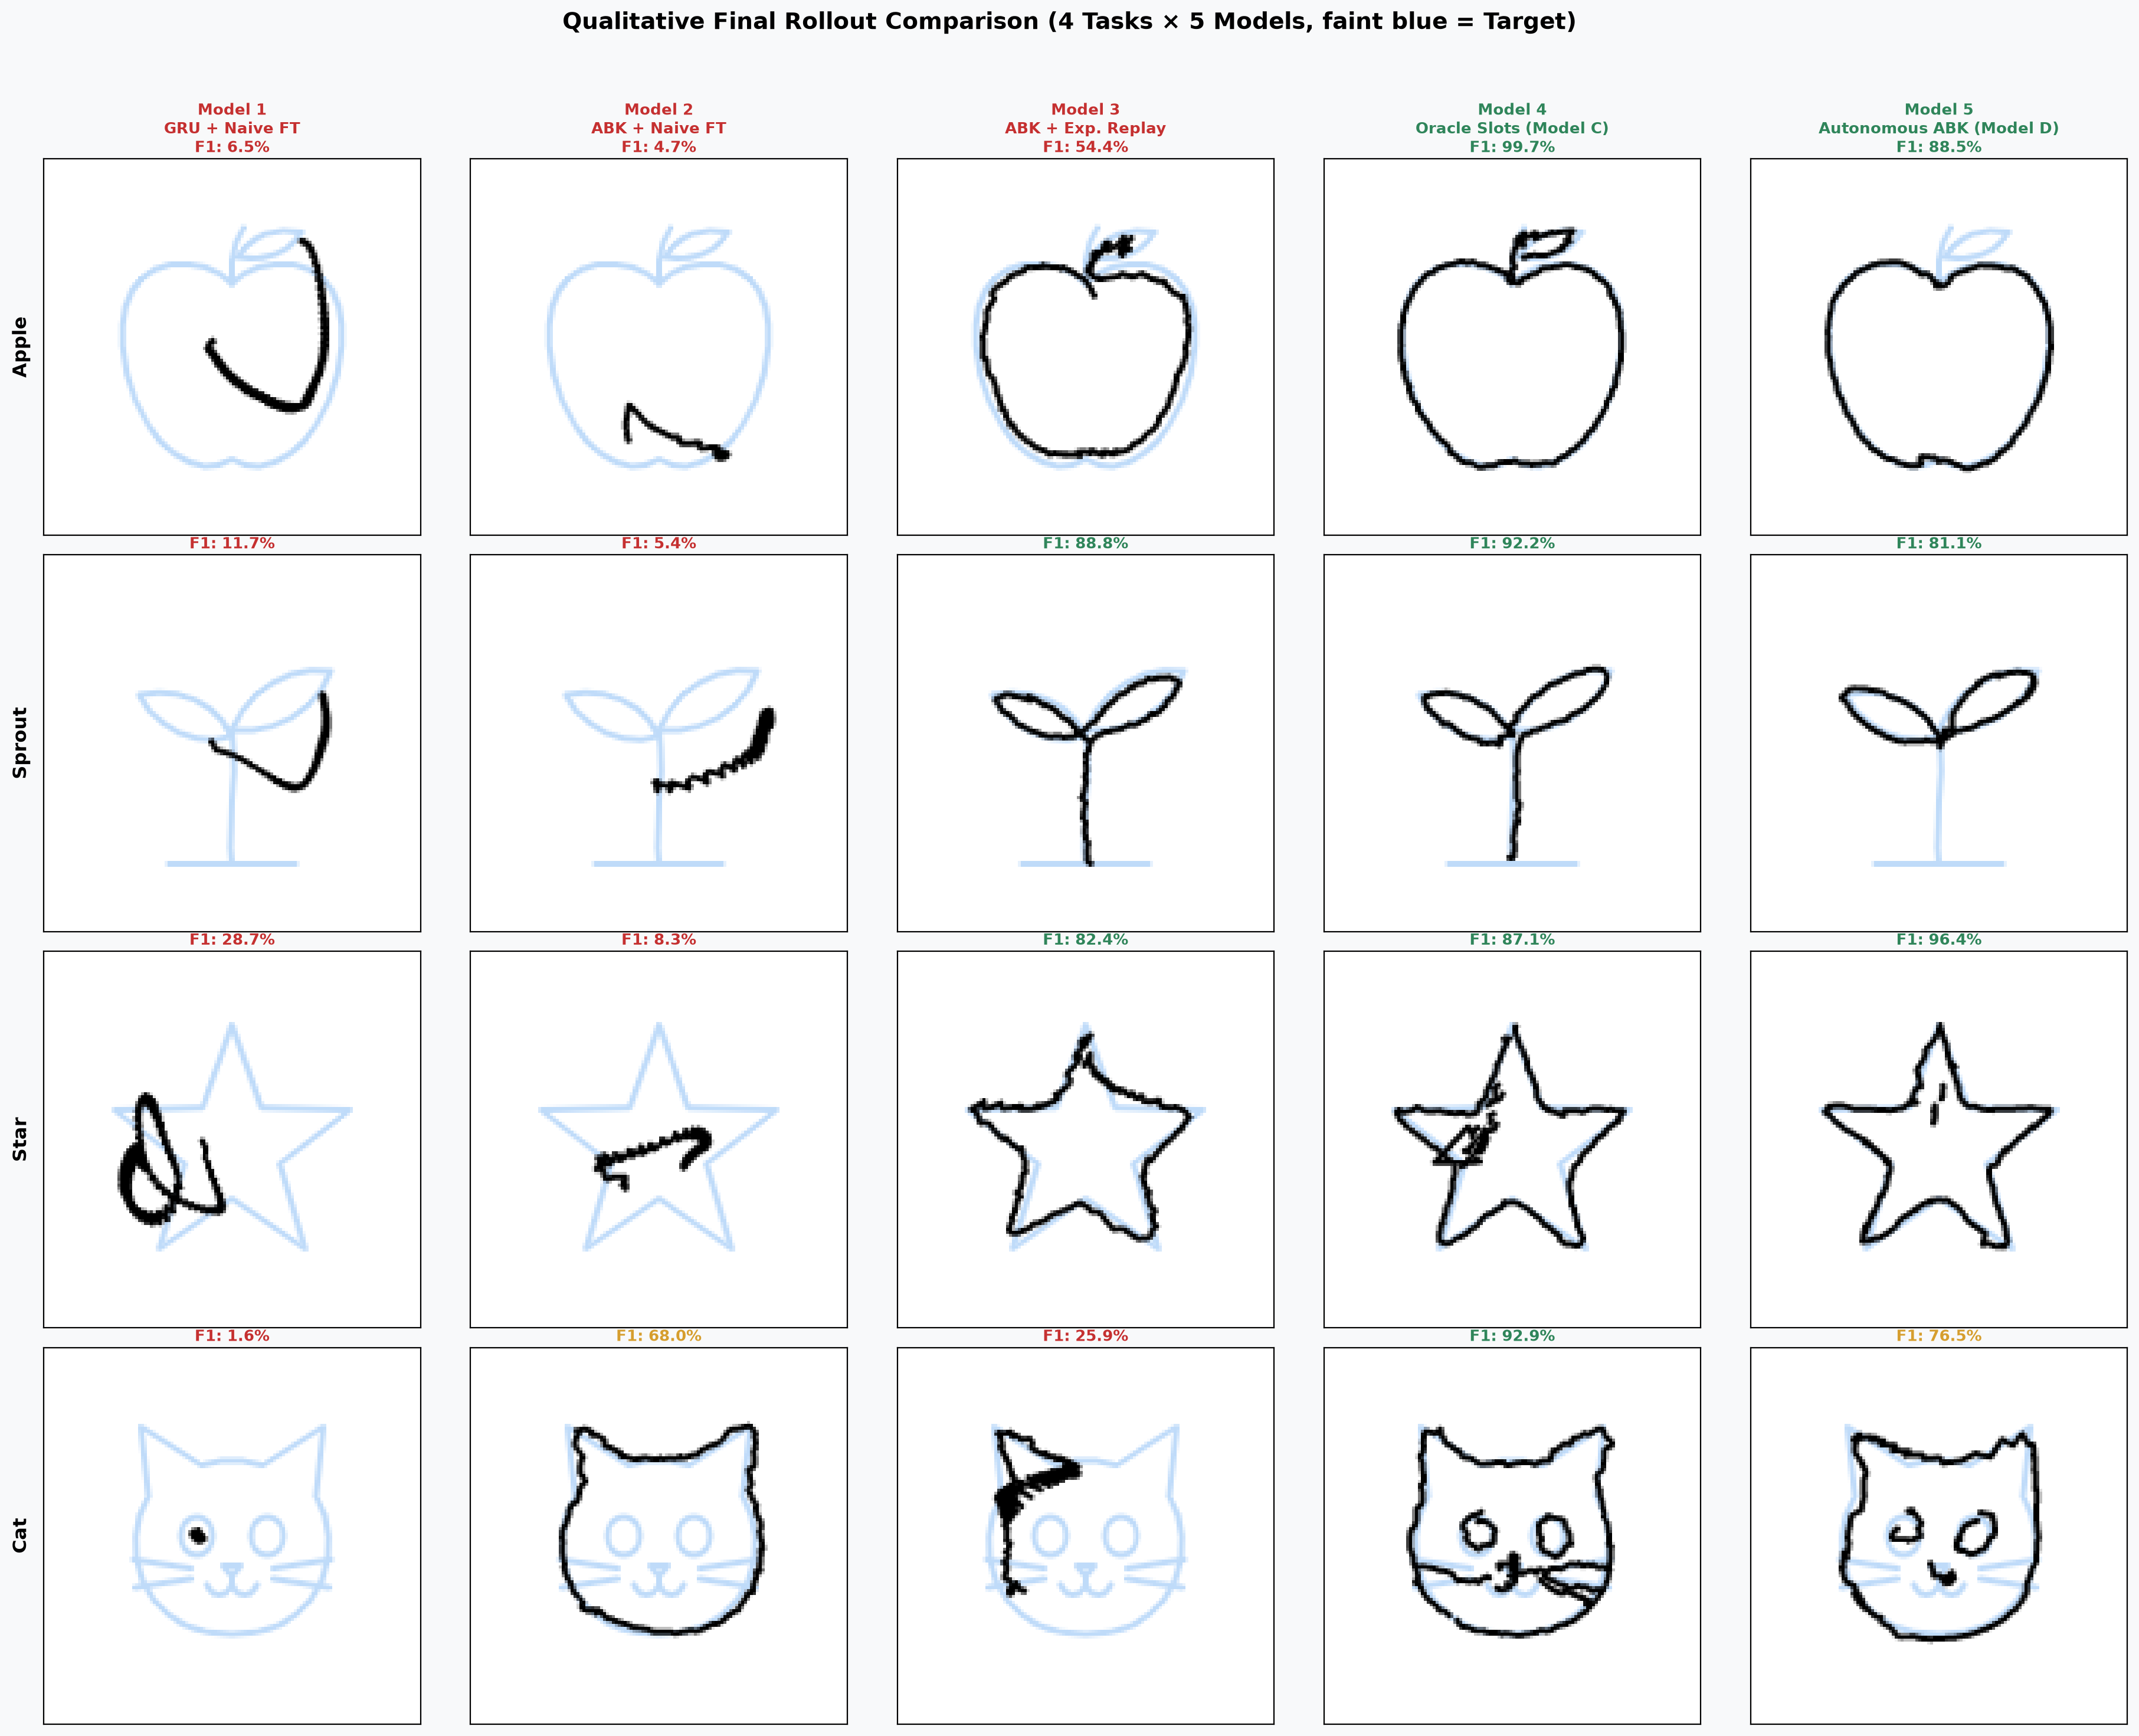
\includegraphics[width=\textwidth]{../outputs/autonomous_cl_rollout_grid.png}
    \caption{\textbf{Qualitative 5-model continual learning rollout comparison} after sequentially learning $\text{apple} \rightarrow \text{sprout} \rightarrow \text{star} \rightarrow \text{cat}$ (faint blue: target outline; black: executed ink). Models~1 and~2 suffer severe trajectory collapse on prior tasks, while Model~3 (Replay) fails on complex multi-part \texttt{Cat} geometry ($25.9\%$). Autonomous ABK-VLA (Model~5) preserves high structural fidelity across all four tasks without test-time \texttt{Task-ID} labels.}
    \label{fig:rollout_grid}
\end{figure*}

\begin{table*}[t]
\centering
\caption{5-Model Continual Learning Benchmark ($T_0:\text{apple} \rightarrow T_1:\text{sprout} \rightarrow T_2:\text{star} \rightarrow T_3:\text{cat}$, \texttt{seed=42}).}
\label{tab:main_benchmark}
\resizebox{\textwidth}{!}{
\begin{tabular}{llccccc}
\toprule
\textbf{Axis} & \textbf{Metric} & \textbf{Model 1} & \textbf{Model 2} & \textbf{Model 3} & \textbf{Model 4 (Oracle)} & \textbf{Model 5 (Ours)} \\
 & & \texttt{GRU + Naive FT} & \texttt{ABK + Naive FT} & \texttt{ABK + Replay} & \texttt{ABK Slots (C)} & \texttt{Autonomous ABK (D)} \\
\midrule
\multirow{2}{*}{\textbf{Conditions}} & Inference \texttt{Task-ID} & None & None & None & Required (Oracle) & \textbf{None (Autonomous)} \\
 & Experience Replay & None & None & 256 / task & None & \textbf{None} \\
\midrule
\multirow{5}{*}{\textbf{Precision ($F_1 \uparrow$)}} & Apple ($T_0$) & 6.5\% & 4.7\% & 54.4\% & \textbf{99.7\%} & 88.5\% \\
 & Sprout ($T_1$) & 11.7\% & 5.4\% & 88.8\% & \textbf{92.2\%} & 81.1\% \\
 & Star ($T_2$) & 28.7\% & 8.3\% & 82.4\% & 87.1\% & \textbf{96.4\%} \\
 & Cat ($T_3$) & 1.6\% & 68.0\% & 25.9\% & \textbf{92.9\%} & 76.5\% \\
 & \textbf{Avg Final $F_1 \uparrow$} & 12.12\% & 21.61\% & 62.87\% & \textbf{92.96\%} & \textbf{85.59\%} \\
\midrule
\multirow{2}{*}{\textbf{Continual Learning}} & \textbf{Forgetting Rate $\downarrow$} & 46.44\% & 89.33\% & 14.13\% & \textbf{0.00\%} & \textbf{1.66\%} \\
 & Backward Transfer (BWT) & -46.44\% & -89.33\% & +1.95\% & 0.00\% & \textbf{-1.66\%} \\
\midrule
\multirow{3}{*}{\textbf{Geometry \& Control}} & \textbf{Chamfer Distance $\downarrow$} & 0.1043 & 0.0984 & 0.0327 & \textbf{0.0098} & \textbf{0.0192} \\
 & \textbf{Normalized Mean Jerk $\downarrow$} & 5.05 & 5.91 & 5.92 & \textbf{3.09} & \textbf{3.33} \\
 & \textbf{Component Recall $\uparrow$} & 0.0\% & 6.3\% & 50.0\% & \textbf{87.5\%} & \textbf{62.5\%} \\
\midrule
\multirow{2}{*}{\textbf{Efficiency}} & Episode Latency (ms) $\downarrow$ & 601.6 ms & 108.6 ms & 564.9 ms & 346.6 ms & \textbf{464.3 ms} \\
 & $T_3$ Trainable Params & 5.08M & 4.72M & 4.72M & 0.30M & \textbf{0.33M (94.44\% Frozen)} \\
\bottomrule
\end{tabular}
}
\end{table*}

\begin{figure*}[t]
    \centering
    \begin{minipage}[t]{0.66\textwidth}
        \centering
        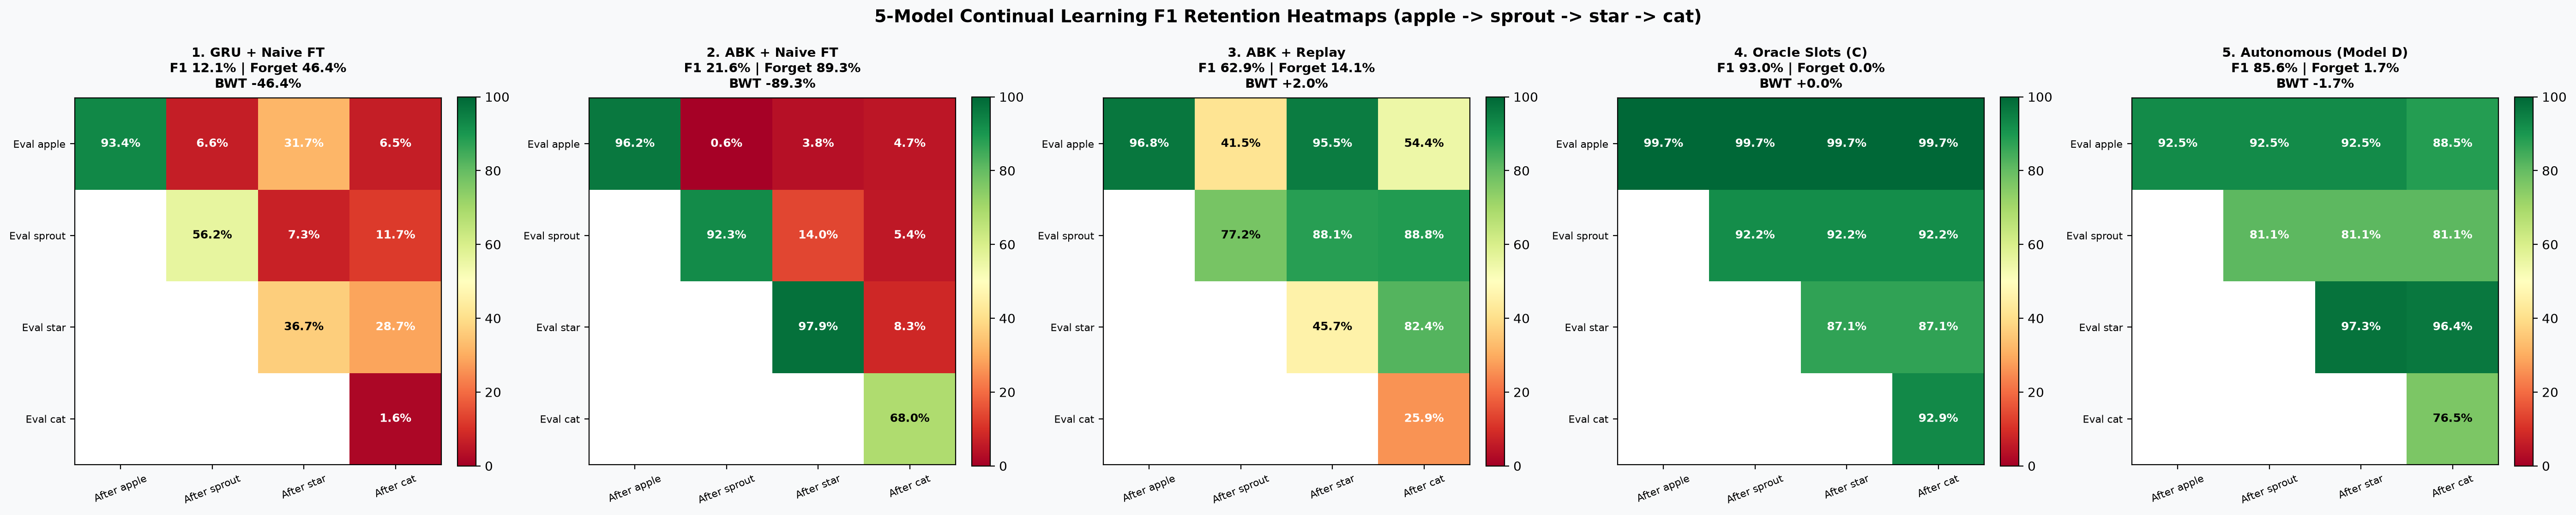
\includegraphics[width=\textwidth]{../outputs/autonomous_cl_heatmap.png}
        \caption{\textbf{Sequential $F_1$ retention heatmaps} across the 4-task curriculum for all five models.}
        \label{fig:heatmap}
    \end{minipage}\hfill
    \begin{minipage}[t]{0.32\textwidth}
        \centering
        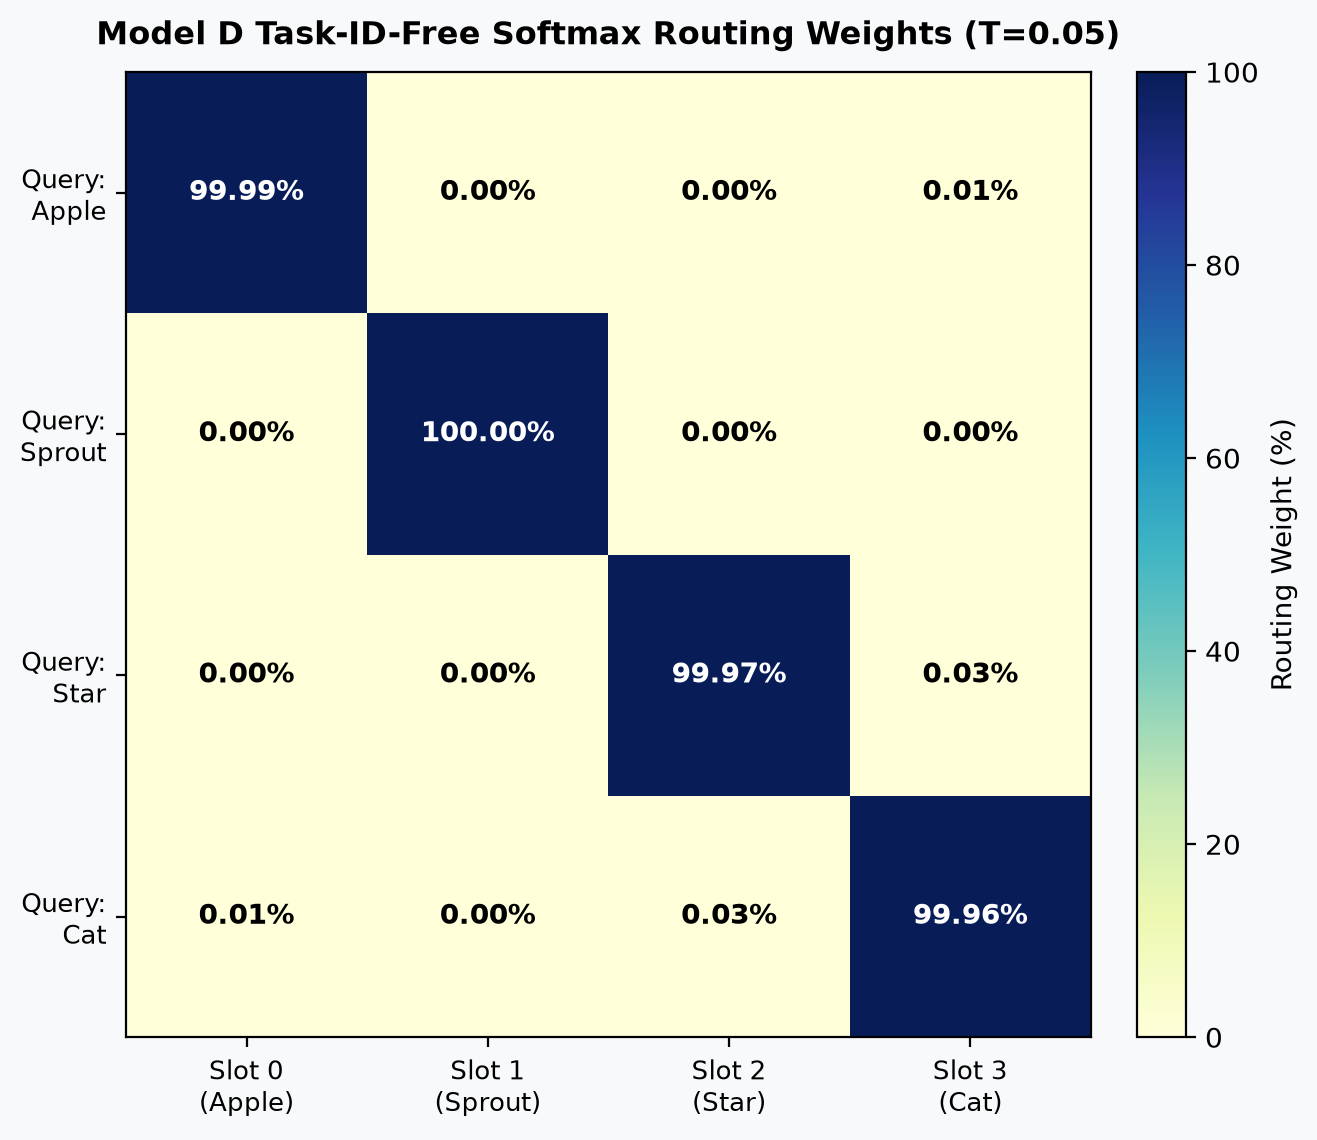
\includegraphics[width=\textwidth]{../outputs/autonomous_routing_matrix.png}
        \caption{\textbf{Task-ID-free softmax routing weights} ($T=0.05$) on canonical target templates.}
        \label{fig:routing}
    \end{minipage}
\end{figure*}

\subsection{Quantitative Comparison}
As shown in Table~\ref{tab:main_benchmark} and Figures~\ref{fig:rollout_grid}--\ref{fig:heatmap}, sequential fine-tuning without isolation suffers severe forgetting: Model~1 (\texttt{GRU + Naive FT}) drops to $12.12\%$ average $F_1$ ($46.44\%$ forgetting, $0.0\%$ component recall), and Model~2 (\texttt{ABK + Naive FT}) exhibits $89.33\%$ forgetting. Experience replay (Model~3) mitigates forgetting ($14.13\%$), but its single-mode predictor trained at $\text{lr}=3\times 10^{-4}$ degrades to $25.9\%$ on multi-part \texttt{Cat} ($62.87\%$ average $F_1$).

In contrast, \textbf{Autonomous ABK-VLA (Model~5)} achieves an average final $F_1$ of \textbf{85.59\%}, recovering \textbf{92.1\%} of the external-\texttt{Task-ID} Model~4 ($92.96\%$) with a forgetting rate of \textbf{1.66\%} ($54.0\times$ lower than Model~2). Geometrically, Model~5 lowers Chamfer Distance to \textbf{0.0192} ($5.4\times$ better than GRU) with smooth trajectories ($\text{NMJ}=3.33$). Note that Model~5 outperforms Model~4 on \texttt{Star} ($96.4\%$ vs.\ $87.1\%$) due to its pointer-conditioned mode selector, focal gating, and residual head ($0.33\text{M}$ vs.\ $0.30\text{M}$). Because Select-then-Blend averages all slots with small residual tail weights ($<0.04\%$) rather than hard \texttt{argmax} gating, adding later slots slightly perturbs frozen earlier rollouts (\texttt{Apple}: $92.48\% \rightarrow 88.46\%$; \texttt{Star}: $97.30\% \rightarrow 96.36\%$), explaining the minor $1.66\%$ forgetting.

\subsection{Autonomous Visual Routing \& Latency Analysis}
Evaluating the temperature-scaled softmax router ($T=0.05$, Figure~\ref{fig:routing}) on the four canonical task target templates yields diagonal routing weights of \texttt{Apple} $\rightarrow$ Slot~0 ($99.99\%$), \texttt{Sprout} $\rightarrow$ Slot~1 ($100.00\%$), \texttt{Star} $\rightarrow$ Slot~2 ($99.97\%$), and \texttt{Cat} $\rightarrow$ Slot~3 ($99.96\%$), giving \textbf{99.98\% mean diagonal confidence} ($4/4$ slot match). At task transitions, novelty detection ($\gamma=0.85$) cleanly triggered expansion with maximum prior similarities of $0.351$ (\texttt{sprout}), $0.491$ (\texttt{star}), and $0.593$ (\texttt{cat}). With static target key caching (\texttt{reset\_cache()}), Model~5 averages \textbf{464.3 ms} per episode ($7.02\text{ ms}$/chunk)---$1.30\times$ faster than GRU ($601.6\text{ ms}$) and $1.22\times$ faster than Replay ($564.9\text{ ms}$), while slower than single-slot Model~4 ($346.6\text{ ms}$) and early-stalling Model~2 ($108.6\text{ ms}$) because Select-then-Blend forwards all $K=4$ slots.

\subsection{Horizon Alignment \& Stall Patience Trade-Off}
Aligning $\text{exec\_steps}=16$ to the full $H=16$ spline horizon preserves pen-up jump landings without truncating airborne chunks prior to touchdown. Under the rollout stall timer (base $\text{patience}=8$, dynamically extended to $16$ when $>5\%$ target ink remains), long air-jumps toward thin auxiliary strokes (e.g., apple leaf, sprout stem, cat whiskers) still occasionally hit stall termination prior to landing ($62.5\%$ component recall vs.\ $87.5\%$ Oracle).

\section{Scope, Limitations, and Future Work}
We explicitly state four scope boundaries of this study:
\begin{enumerate}
    \item \textbf{Goal-Image-Conditioned Scope:} ABK-VLA here denotes a compact goal-image-conditioned visuomotor action-chunking policy on a 2D drawing testbed; the current implementation contains no language encoder or VLM/LLM backbone.
    \item \textbf{Training Task Boundaries:} While inference is \texttt{Task-ID}-free, sequential training invokes \texttt{register\_or\_expand\_slot} at discrete task loader boundaries.
    \item \textbf{Canonical Prototype Evaluation:} Because the $5{,}376$-d key devotes $80\%$ of its squared $L_2$ norm to spatial target pooling and the $99.98\%$ routing matrix is evaluated on the four canonical static target templates themselves (self-similarity $=1.0$), evaluating routing under affine-perturbed or noisy OOD target queries remains future work.
    \item \textbf{Linear Slot Scaling \& Single-Seed Run:} Select-then-Blend incurs $O(K)$ parameters and forward passes per step ($5.90\text{M}$ total at $T_3$), and all benchmark numbers are from a single-seed (\texttt{seed=42}), single-order run; replacing soft blending with hard \texttt{argmax} gating could eliminate the remaining $1.66\%$ forgetting.
\end{enumerate}

\section{Conclusion}
ABK-VLA shows that pairing cubic B-spline trajectory compression with residual WTA slots and visual prototype routing enables compact visuomotor policies to achieve $85.59\%$ average $F_1$, $1.66\%$ forgetting, and $99.98\%$ diagonal routing confidence on canonical targets without replay buffers or test-time \texttt{Task-ID} labels.

\begin{thebibliography}{9}
\bibitem{kirkpatrick2017} J. Kirkpatrick et al., ``Overcoming catastrophic forgetting in neural networks,'' \textit{PNAS}, vol. 114, no. 13, pp. 3521--3526, 2017.
\bibitem{rusu2016} A. A. Rusu et al., ``Progressive neural networks,'' \textit{arXiv:1606.04671}, 2016.
\bibitem{zhao2023} T. Z. Zhao et al., ``Learning fine-grained bimanual manipulation with low-cost hardware,'' \textit{RSS}, 2023.
\bibitem{farquhar2018} S. Farquhar and Y. Gal, ``Towards robust evaluations of continual learning,'' \textit{arXiv:1805.09733}, 2018.
\end{thebibliography}

\end{document}
